% !TeX program = PdfLaTeX
% !TeX root = ../Main.tex

\chapter{Theoretical background}
\label{ch:ch2} %serve per citare il capitolo in un'altra sezione

Takeoff speeds are a safety key element for takeoff, and enable pilot situational
awareness and decision-making in this very dynamic situation. The use of erroneous
takeoff speeds can lead to tail strikes, high-speed rejected takeoff or initial climb with
degraded performance. 

% --------------------------------------------------------------------------------------------------------------------------------------------
% 								SEZIONE 1
% --------------------------------------------------------------------------------------------------------------------------------------------

\section{Take off speeds}
In this section a brief introduction to takeoff speeds will be provided \cite{Airbus:Flight:Notes}. \\
In aviation, these speeds are standard terms used to define airspeeds important or useful to the operation of all aircraft. They are derived from data obtained by aircraft designers and manufacturers during flight testing and verified in most countries by government flight inspectors during aircraft type-certification testing. Using them is considered a best practice to maximize aviation safety, aircraft performance or both. Takeoff speeds are calculated prior to a take off in accordance with aircraft weight, environmental factors etc.

\begin{figure}[htbp]
	\centering
	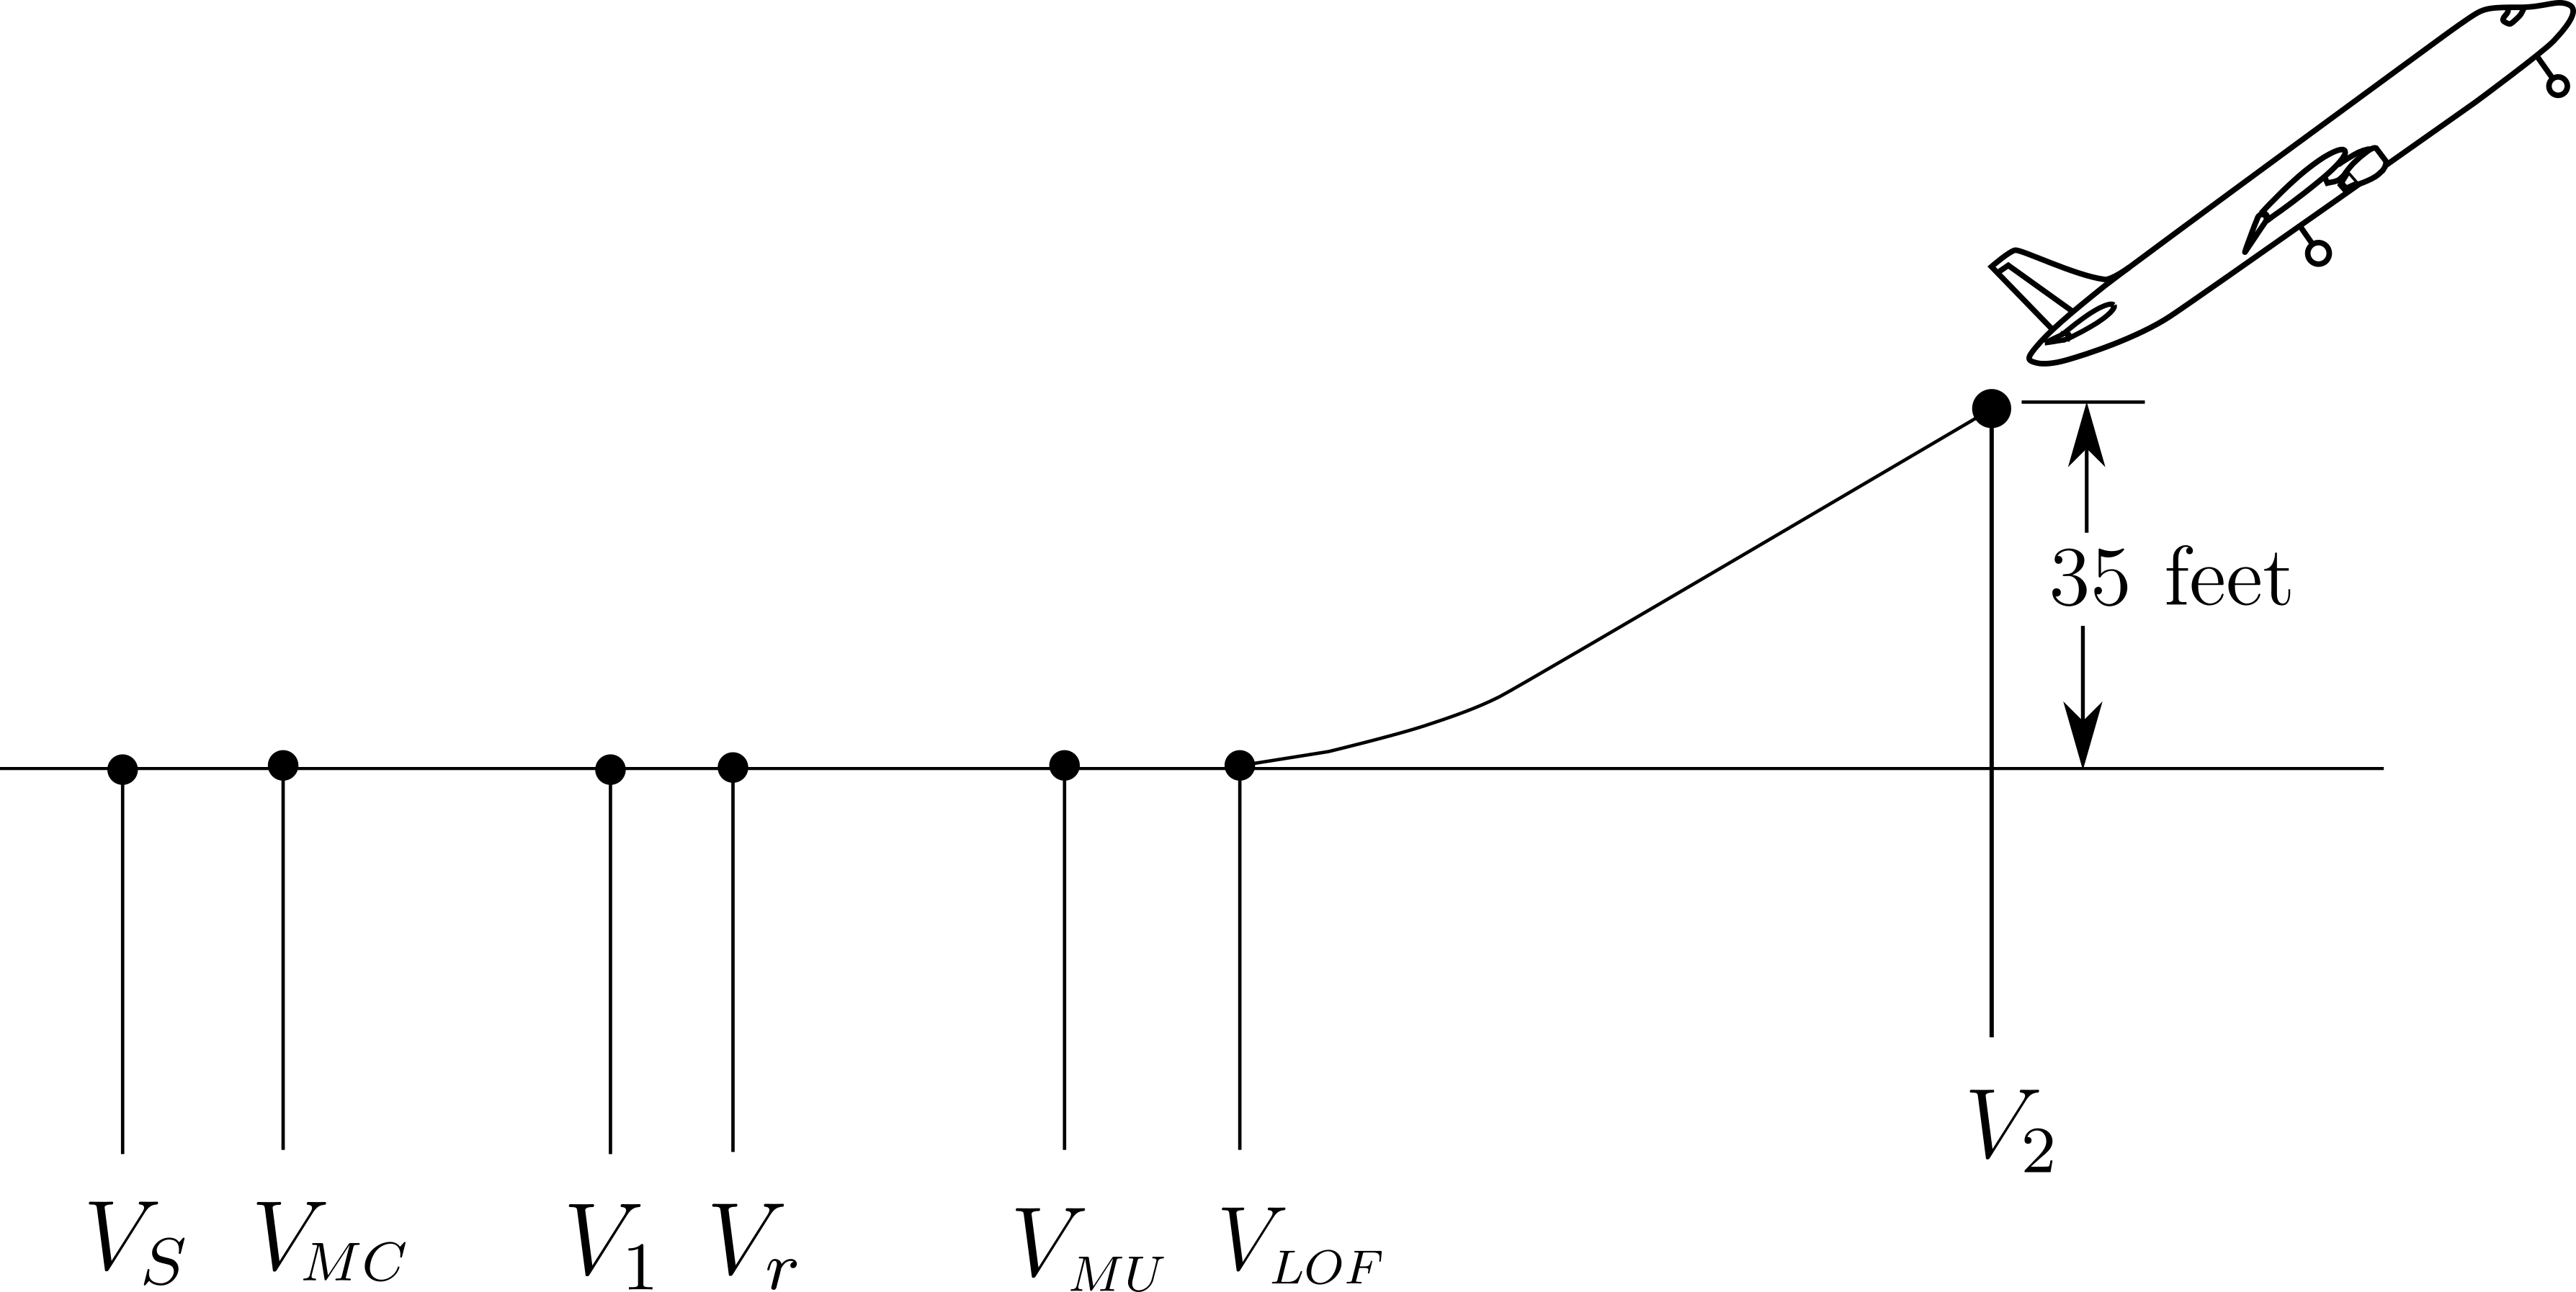
\includegraphics[height=7cm, keepaspectratio ]{Immagini/Capitolo2/takeoffSpeeds} 
	\caption{Takeoff speeds} % didascalia
	\label{fig:figura2_4} % etichetta per citarla nel testo
\end{figure}

\subsubsection{Velocity of stall $V_{S}$}
Aircraft stall speed during take off run.

\subsubsection{Velocity of Minimum Control $V_{MC}$}
During the takeoff roll, it is of utmost importance to know the minimum speed at which
the aircraft will remain controllable, in the event of an engine failure on ground. This is
because, in such a case, and if the takeoff is continued, only the rudder will be able to
counteract the yaw moment that is generated by asymmetric engine(s) thrust.
According to current regulations, the minimum speed at which an aircraft is defined to be “controllable”
(lateral excursion lower than 30 feet) after an engine failure on ground, is referred to
as $V_{MC}$ (Velocity of Minimum Control on Ground). 

\subsubsection{Decision Speed $V_1$}
$V_1$ is the maximum speed at which a rejected takeoff can be initiated, in the event of an
emergency. $V_1$ is also the minimum speed at which a pilot can continue a takeoff after an engine
failure.
If an engine failure is detected after $V_1$, the takeoff must be continued. This implies that
the aircraft must be controllable on ground. Therefore, V1 is always greater than $V_{MC}$.

\subsubsection{Rotation speed $V_r$}
Speed at which planes with a tricycle trolley lift the front wheel off the ground during take off.
 
\subsubsection{Velocity of Minimum Unstick $V_{MU}$}
 $V_{MU}$ is achieved by pitching the aircraft up to the maximum (tail on the runway, for
aircraft that are are geometrically-limited) during the takeoff roll (Refer to Figure~\ref{fig:figura2_1}). The speed at which the aircraft first lifts off is  $V_{MU}$. Therefore, lift-off is not
possible prior to  $V_{MU}$. 

\begin{figure}[htbp]
	\centering
	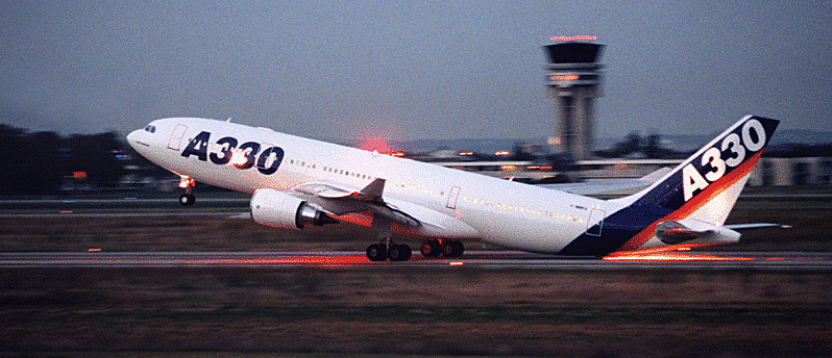
\includegraphics[height=6cm, keepaspectratio ]{Immagini/Capitolo2/2_1-VMUFlightTestOnAnA330} 
	\caption{$V_{MU}$ Flight Test on an Airbus A330} % didascalia
	\label{fig:figura2_1} % etichetta per citarla nel testo
\end{figure}

\subsubsection{Lift-off speed $V_{LOF}$}
Effective take off speed. It is assessed by adding a 10\% to the Minimum unstick speed with all the operating engines or a 5\% with an inoperative engine.

\subsubsection{Takeoff safety speed $V_2$}
$V_2$ is the speed at which the aircraft may safely be climbed with one engine inoperative. This speed is nicknamed a “take off safety speed”; it is the speed an aircraft with one engine inoperative must be able to attain in order to leave the runway and get 35 feet off the ground at the end of the runway, maintaining a 200 ft/min climb thereafter. This is the lowest speed at which the aircraft complies with the handling criteria associated with a climb after a take off, followed by the failure of an engine.

% --------------------------------------------------------------------------------------------------------------------------------------------
% 								SEZIONE 2	
% --------------------------------------------------------------------------------------------------------------------------------------------

\section{Ground effect}
Due to the fact that during the takeoff the aircraft is on the ground, in order to asses $V_{MU}$,  it is important to consider the ground effect. This generally become measurable at a height above the ground of one wing-span and increase in magnitude as the height above the ground decreases. Both theoretical and
experimental investigations indicate that ground proximity produces an increase in the lift-curve
slope, a decrease in drag, and a reduction of nose-up pitching moment for most aircraft planforms in
the clean configuration. However, high-lift configurations deviate from this trend in that the ground
effect tends to reduce the lift-curve slope \cite{Datcom}.\\

The majority of the theoretical approaches analyzing ground effects employ an image-vortex theory
to represent the ground plane. The salient aspects of this theory are discussed below.\\

Away from the ground plane, the downwash of the two trailing vortices contributes to the wing
drag die to lift by rotating the force vector rearward.\\
However, near the ground plane, the trailing vortices of the image vortex system have an upwash component.\\

This upwash velocity component reduces the downward rotation of the flow direction caused by the wing trailing vortices, thus decreasing the wing drag due to lift.\\

The ground effects on lift are determined somewhat by the planform of the configuration. For
low-aspect-ratio delta configurations, the general trend is a constant increase in $C_L$ due to ground
effect, as shown in figure~\ref{fig:figura2_2}.
However, transport-type configurations show quite a different trend, as presented in figure~\ref{fig:figura2_3}.\\
This trend is dependent upon tie type of high-lift system employed.

\begin{figure}[htbp]
	\centering
	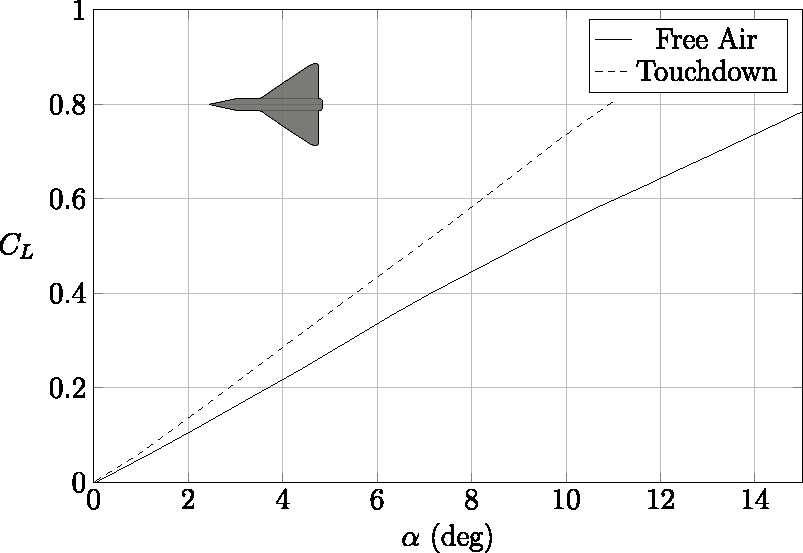
\includegraphics[height=10cm, keepaspectratio ]{Immagini/Capitolo2/2_2-GroundEffectDeltaConf} 
	\caption{Ground effect on 55°  delta configuration} % didascalia
	\label{fig:figura2_2} % etichetta per citarla nel testo
\end{figure}

\begin{figure}[htbp]
	\centering
	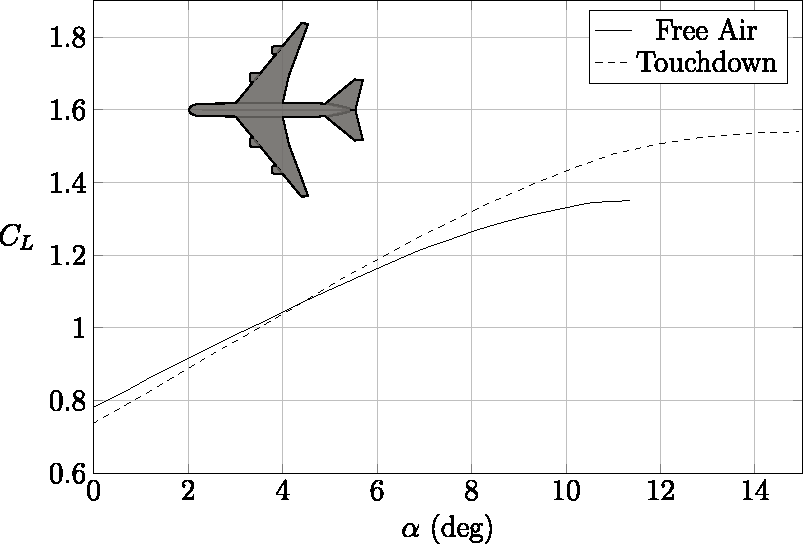
\includegraphics[height=10cm, keepaspectratio ]{Immagini/Capitolo2/2_3-GroundEffectJetTranspConf} 
	\caption{Ground effect on a jet transport configuration} % didascalia
	\label{fig:figura2_3} % etichetta per citarla nel testo
\end{figure}

\section{Datcom methods}
\label{sec:sec3}
For most vehicles, calculating the change in lift due to ground effects consists of evaluating two
components:
 \begin{enumerate}
 \item the change in wing-body lift;
 \item the change in tail-body lift due to the effects of downwash.
 \end{enumerate}
 
The change in tail-body lift due to the presence of the ground is generally small in comparison to
the downwash effects and is neglected in the Datcom methods.\\
Both of the Datcom methods presented require the user to construct wing-body and tail-body lift
curves in ground effect based on their corresponding free-air lift curves. Equations are given that
calculate the change in angie of attack due to ground effect at a constant lift coefficient. The
ground-effect lift curves are then constructed by shifting the free-air lift curves at every $C_L$ by the
corresponding increment in angle of attack due to ground effect at constant lift coefficients.

\begin{figure}[htbp]
	\centering
	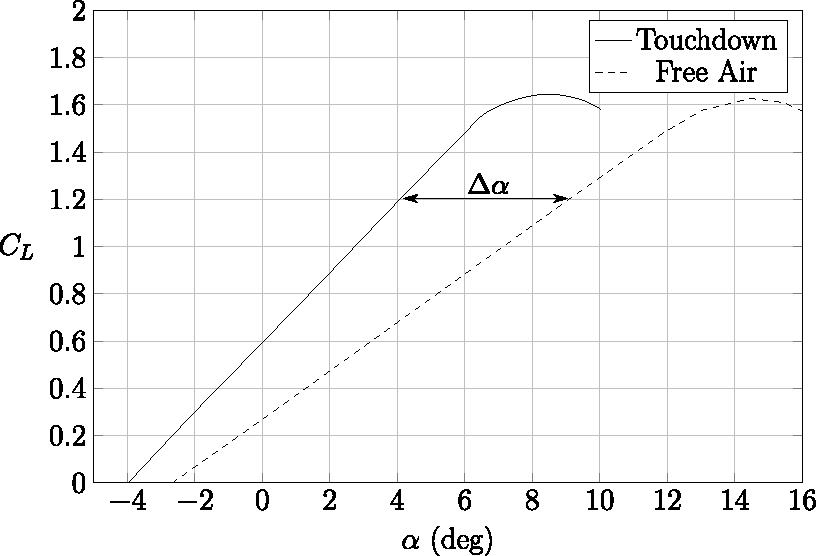
\includegraphics[height=10cm, keepaspectratio ]{Immagini/Capitolo2/disegno} 
	\caption{Ground effect on a jet transport configuration} % didascalia
	\label{fig:figura2_3_1} % etichetta per citarla nel testo
\end{figure}

\subsubsection{Method I}
This method estimates the ground effects on lift in the linear-lift range for a subsonic transport
configuration. It includes the effects of taper ratio, sweep-back, dihedral, and flap deflection, while neglecting the effects of
wing thickness since they are generally small. The wing-flap effects are valid only for split and slotted flaps as they are accounted for by empirical curves. \\
The change in wing-body angle of attack at a constant lift coefficient due to ground effect with
respect to the out-of-ground-effect lift curve is given by:

\begin{equation}
\begin{split}
\left(\Delta \alpha\right)_G=&-\left[\frac{9.12}{\AR}+7.16\left(\frac{c_r}{b}\right)\right]\left( C_{L_f} \right)_{WB}x \ +\\
&-\frac{\AR}{2\left( C_{L_{\alpha}} \right)_{WB}}\left(\frac{c_r}{b}\right)\left(\frac{L}{L_0}-1\right)\left( C_{L_f} \right)_{WB}r \ + \\ &-\frac{\left(\delta_f /50\right)^2}{\left( C_{L_{\alpha}} \right)_{WB}}\Delta \left(\Delta C_L \right)_{flap} \ \text{(per  deg)}
\label{eq:equazione2_1} % etichetta per citarla nel testo
\end{split}
\end{equation}
\\ \\ \\ \\  where\\ \\ \\
\begin{tabulary}{1\textwidth}{L L}
\begin{minipage}[T]{6cm}$\Delta \left(\Delta C_L \right)_{flap}$  \end{minipage}& is an empirical factor to account for the effect of flaps and is obtained from~\vref{fig:figura2_4} as a function of the height of the quarter-chord point of the wing root chord above the ground,\\ \\
\AR & is the wing aspect ratio, \\ \\
$\dfrac{c_r}{b}$ & is the ratio of wing root chord to wing span, \\ \\
$\left( C_{L_f} \right)_{WB} $ & is the wing-body lift coefficient including flap effects, out of ground effect, \\ \\
$x$ & accounts for the effects on lift due to the image trailing vortex and is obtained
from~\vref{fig:figura2_6} as a function of wing geometry and the wing height above
the ground, \\ \\
$\dfrac{L}{L_0}-1 $ & accounts for the effects on lift due to the image bound vortex and is obtained from~\vref{fig:figura2_8} as a function of wing geometry, lift coefficient, and the height of the quarter-chord point of the wing root chord above the ground. \\ \\
$\left( C_{L_{\alpha}} \right)_{WB} $  & is the wing body lift-curve slope, per degree, out of  ground effect \\ \\
$r$ & accounts for the effect of finite span and is obtained from~\vref{fig:figura2_9} as a function of wing height above the ground, \\ \\
\end{tabulary}

The first term in Equation~\ref{eq:equazione2_1} accounts for the effects of he trailing vortex, the second term for the effects of the trailing vortex, the second term for the effects of the bound vortex, and the third term for wing-flap effects. The method does not account for the effects of wing-leading-edge devices.\\
\begin{figure}[H]
	\centering
	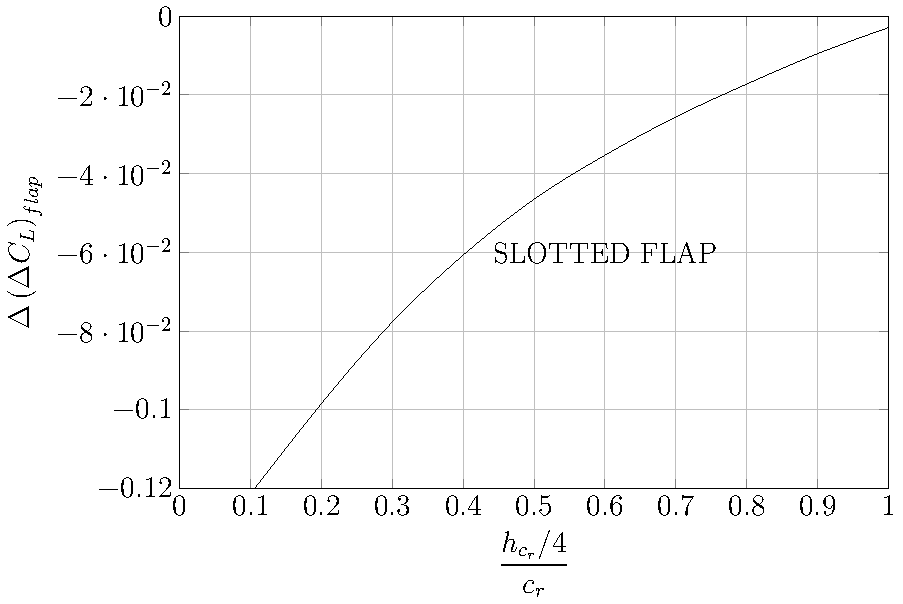
\includegraphics[height=7.3cm, keepaspectratio ]{Immagini/Capitolo2/2_4-Delta_alpha_CL_Ground_Effect_DeltaDelta_CL_flap_vs_h_cr_4_cr} 
	\caption{Effect of flap deflection on the ground influence on lift} % didascalia
	\label{fig:figura2_4} % etichetta per citarla nel testo
\end{figure}

\begin{figure}[H]
	\centering
	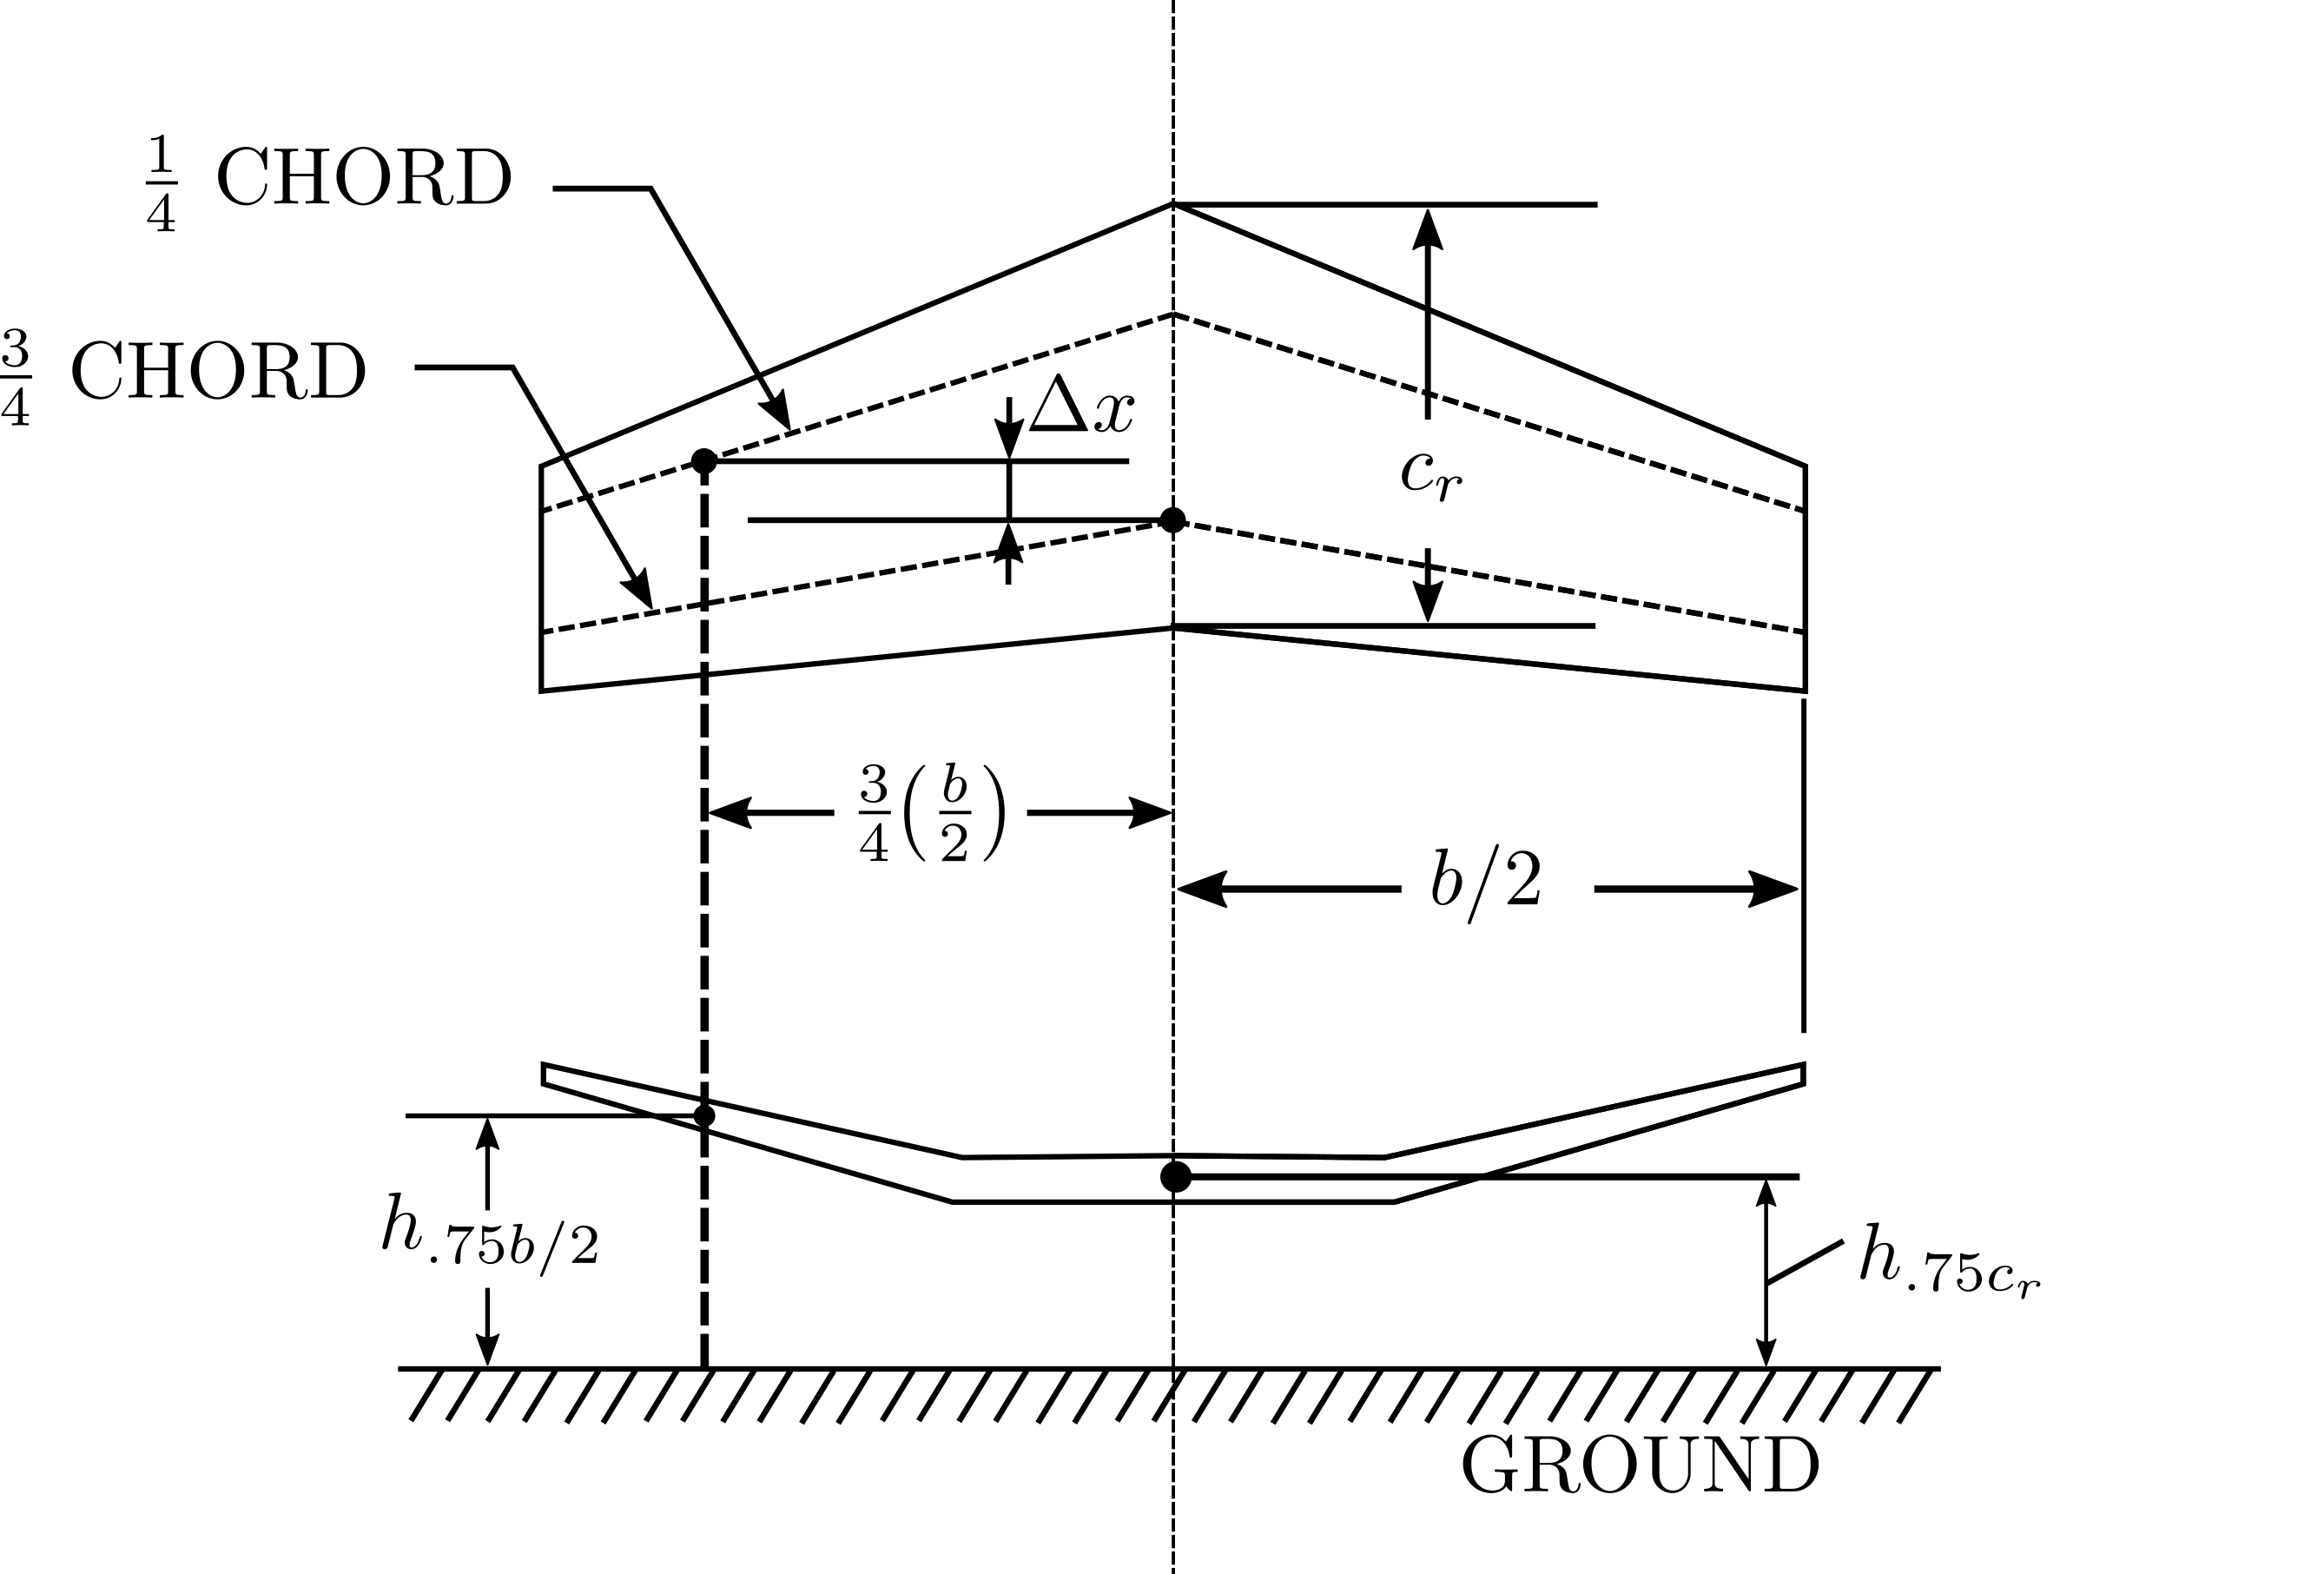
\includegraphics[height=9cm, keepaspectratio ]{Immagini/Capitolo2/disegno-1} 
	\caption{Description of geometric parameters} % didascalia
	\label{fig:figura2_5} % etichetta per citarla nel testo
\end{figure}

where
\[\frac{h}{b/2}=\frac{0.5\left(h_{.75b/2}+h_{.75c_r}\right)}{b/2}\]

\begin{figure}[H]
	\centering
	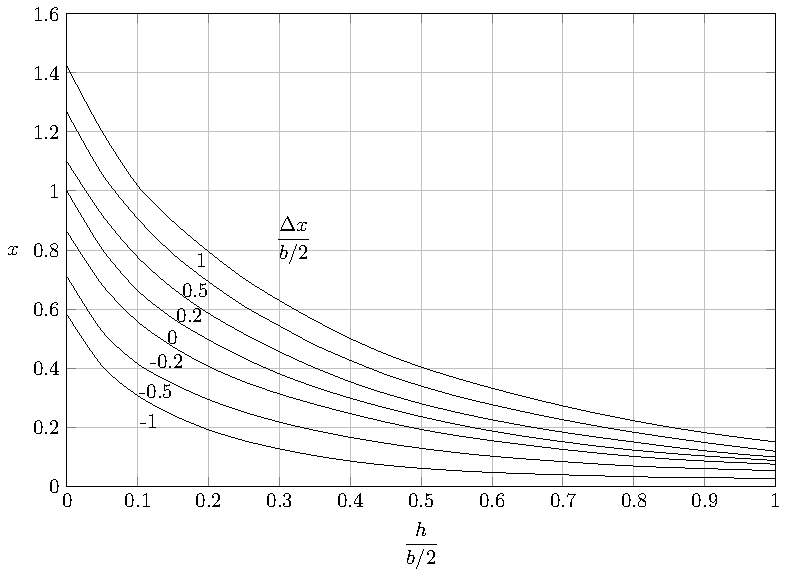
\includegraphics[height=9.5cm, keepaspectratio ]{Immagini/Capitolo2/2_6-(Delta_alpha_CL_Ground_Effect)_x_vs_2hfracb_Deltax} 
	\caption{Parameter accounting for ground effect on lift due to trailing vortices} % didascalia
	\label{fig:figura2_6} % etichetta per citarla nel testo
\end{figure}


\begin{figure}[H]
	%\centering
	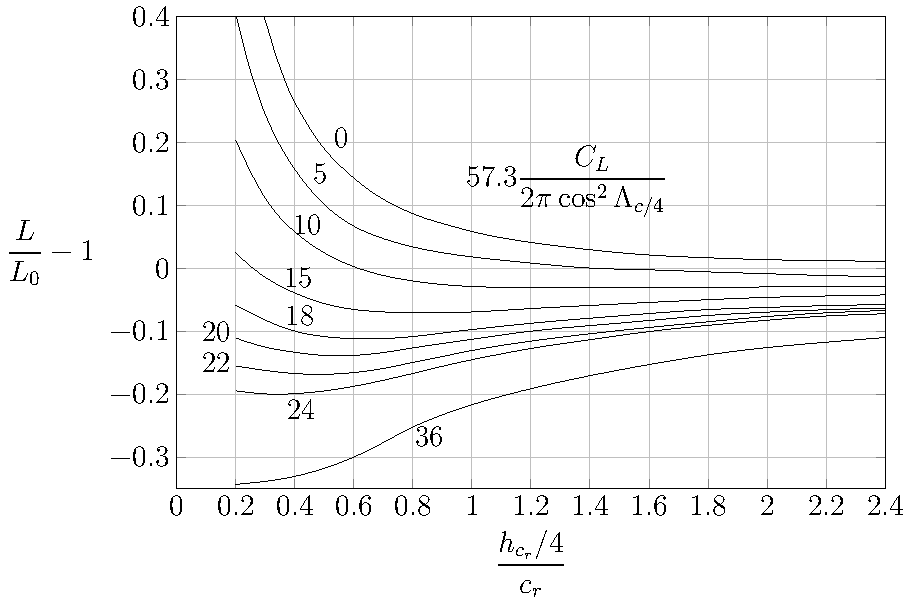
\includegraphics[height=8.5cm, keepaspectratio ]{Immagini/Capitolo2/2_8-Delta_alpha_CL_Ground_Effect_L_L0_minus1_vs_h_cr_4_cr} 
	\caption{Parameter accounting for ground effect on lift due to bound vortices} % didascalia
	\label{fig:figura2_8} % etichetta per citarla nel testo
\end{figure}

\begin{figure}[H]
	\centering
	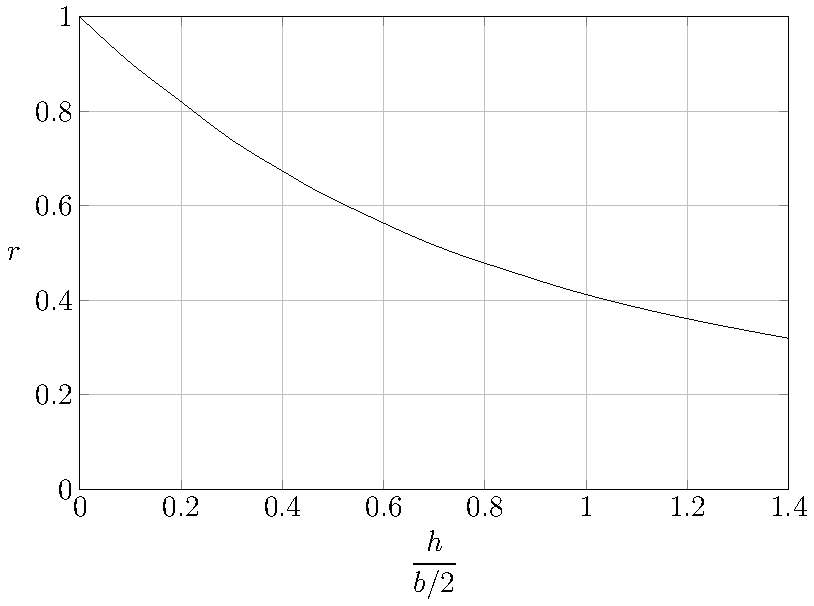
\includegraphics[height=8.5cm, keepaspectratio ]{Immagini/Capitolo2/2_9-Delta_alpha_G_r_vs_2hfracb} 
	\caption{Factor accounting for finite span in ground effect} % didascalia
	\label{fig:figura2_9} % etichetta per citarla nel testo
\end{figure}

In the linear-lift region, the change in downwash (a decrease) on this tail-body due to ground effects
is derived theoretically by representing the ground plane as an image-vortex system.\\
The change (a decrease) in tail-body downwash due to ground effects in the linear-lift range is given by:

\begin{equation}
\left(\Delta \varepsilon \right)_G=\varepsilon \left[\frac{b_{eff}^2+4\left(H_H+H\right)^2}{b_{eff}^2+4\left(H_H-H\right)^2}\right]
\label{eq:equazione2_2} % etichetta per citarla nel testo
\end{equation}
where \\ \\

\begin{tabulary}{1\textwidth}{L L}
\begin{minipage}[T]{3cm}$\left(\Delta \varepsilon \right)_G$  \end{minipage}& is the difference between the downwash in free air and the downwash in
ground effect,\\ \\
$\varepsilon$ & is the downwash out of ground effect, \\ \\
$H$ & is the height of $\frac{\overline c}{4}$ of the wing above the ground, \\ \\
$H_H$ & is the height of $\frac{\overline c}{4}$ of the horizontal tail above the ground.\\ \\
$b_{eff}$ & is the effective wing span defined as\\ \\
\end{tabulary}

\begin{equation}
b_{eff}=\frac{ C_{L_{WB}} +\Delta C_{L_f} }{\dfrac{ C_{L_{WB}} }{b'_W}+ \dfrac {\Delta C_{L_f} }{b'_f}}
\label{eq:equazione2_2_1} % etichetta per citarla nel testo
\end{equation}
  \indent \indent \indent  where \\ \\

\begin{tabulary}{1\textwidth}{L L}
\begin{minipage}[T]{4cm}$\qquad \qquad  C_{L_{WB}}$  \end{minipage}&  is the wing-body lift coefficient, flaps retracted, out of ground effect,\\ \\
$\qquad \qquad  \Delta C_{L_f}$ & is the change in lift coefficient due to flaps, out of ground effect. \\ \\
\end{tabulary}

\begin{equation}
b'_W=\left(\frac{b'_W}{b}\right)b
\label{eq:equazione2_3_1} % etichetta per citarla nel testo
\end{equation}

\begin{equation}
b'_W=\left(\frac{b'_f}{b'_W}\right)\left(\frac{b'_W}{b}\right)b
\label{eq:equazione2_3_2} % etichetta per citarla nel testo
\end{equation}
 \indent \indent \indent The ratio $\dfrac{b'_W}{b}$ is given in~\vref{figura2_10} as a function of taper \indent \indent \indent ratio and aspect ratio, and $\dfrac{b'_f}{b'_W}$ is given in~\vref{fig:figura2_11} as   \indent \indent \indent a function of the  ratio  of flap span to wing span.\\
 
The horizontal-tail lift curve in ground effect is constructed by shifting the free-air lift curve at
every $C_L$ by the corresponding \(-\left(\Delta \varepsilon \right)_G\), i.e.,
\begin{equation}
\left(\Delta \alpha_H \right)_G=-\left(\Delta \varepsilon \right)_G
\label{eq:equazione2_3} % etichetta per citarla nel testo
\end{equation}

 \begin{figure}[H]
	%\centering
	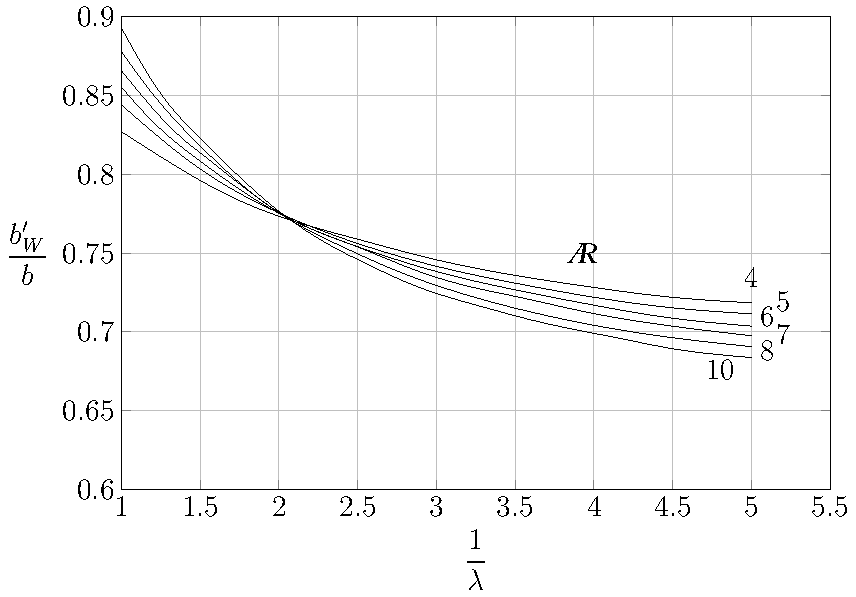
\includegraphics[height=10.5cm, keepaspectratio ]{Immagini/Capitolo2/2_10-bapexwfracb} 
	\caption{Effective wing span in the presence of the ground} % didascalia
	\label{figura2_10} % etichetta per citarla nel testo
\end{figure}

\begin{figure}[H]
	\centering
	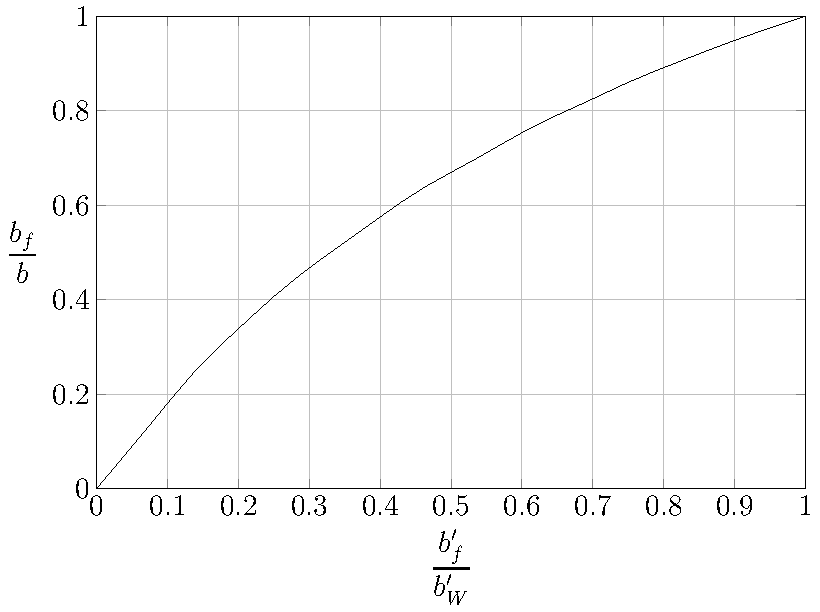
\includegraphics[height=10.5cm, keepaspectratio ]{Immagini/Capitolo2/2_11-bapexffracbapexw} 
	\caption{Effective flap span in the presence of the ground} % didascalia
	\label{fig:figura2_11} % etichetta per citarla nel testo
\end{figure}

\subsubsection{Method II}
This method estimates the ground effects on wing-body lift in the linear-lift range for all
configurations not included in Method I.
The change in wing-body angle of attack due to ground
effects with respect to the out-of-ground-effect lift curve is given by:

\begin{equation}
\left(\Delta \alpha\right)_G=-18.4\frac{\left( C_{L_f} \right)_{WB}\sigma}{\AR}+rT\frac{\left( C_{L_f} \right)_{WB}^2}{57.3\left( C_{L_{\alpha}} \right)_{WB}}-rB+K\left(\frac{t}{c}\right)_{max} \ \text{(per  deg)}
\label{eq:equazione2_4} % etichetta per citarla nel testo
\end{equation}
\\ \\   where\\ \\ \\
\begin{tabulary}{1\textwidth}{L L}
\begin{minipage}[T]{6cm}$\sigma$  \end{minipage}& is Prandtl's interference coefficient from multiplane theory and is obtained from~\vref{fig:figura2_12} as a function of wing height above the ground,\\ \\
$r$ & accounts for the effect of finite span and is obtained from~\vref{fig:figura2_9} as a function of wing height above the ground, \\ \\
$T$ & accounts for the reduction of the longitudinal velocity and is obtained from~\vref{fig:figura2_13} as a function of wing height above the ground, \\ \\
$B$ &accounts for the change in circulation and is obtained from~\vref{fig:figura2_14} as a function of wing height above the ground, \\ \\
$K$ & accounts for the effective wing thickness and is obtained from~\vref{fig:figura2_15} as a function of wing height above the ground, \\ \\
$\left(C_{L_{\alpha}} \right)_{WB}$ & is the wing-body lift-curve slope, per degree, out of ground effect, \\ \\
$\left(\dfrac{t}{c}\right)_{max}$  & is the ratio of maximum wing thickness to wing chord, \\ \\
$\left( C_{L_f} \right)_{WB}$ & is the wing-body lift coefficient including flap effects, out of ground effect. \\ \\
\end{tabulary}

\begin{figure}[H]
	\centering
	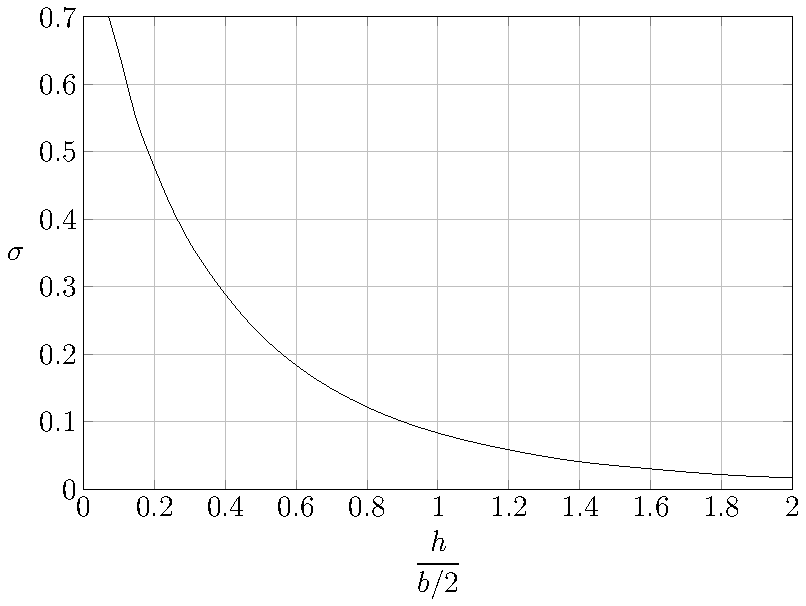
\includegraphics[height=10.5cm, keepaspectratio ]{Immagini/Capitolo2/2_12-(Delta_alpha_G)_sigma_vs_2hfracb} 
	\caption{Prandtl's interference coefficient - indicative of variation in induced vertical velocity with ground effect} % didascalia
	\label{fig:figura2_12} % etichetta per citarla nel testo
\end{figure}

\begin{figure}[H]
	\centering
	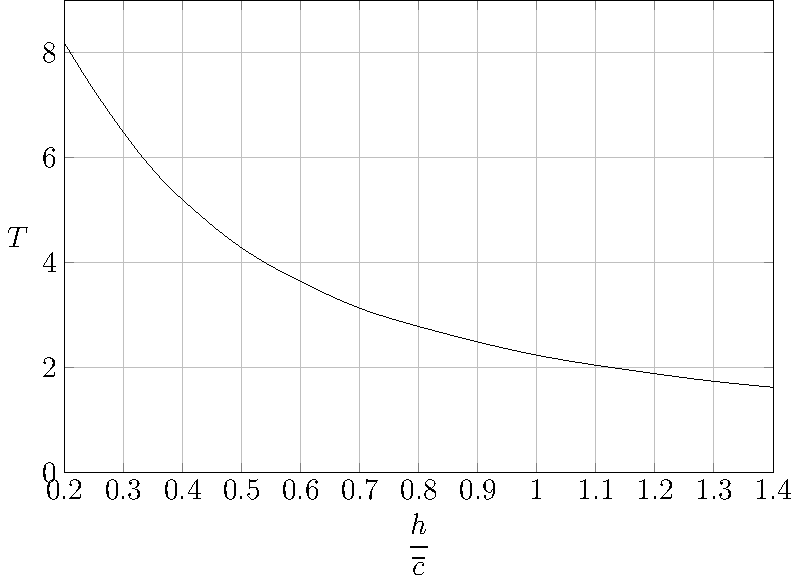
\includegraphics[height=10.5cm, keepaspectratio ]{Immagini/Capitolo2/2_13-(Delta_alpha_G)_T_vs_h_frac_overline_c} 
	\caption{Parameter accounting for variation in longitudinal velocity with ground height} % didascalia
	\label{fig:figura2_13} % etichetta per citarla nel testo
\end{figure}

\begin{figure}[H]
	%\centering
	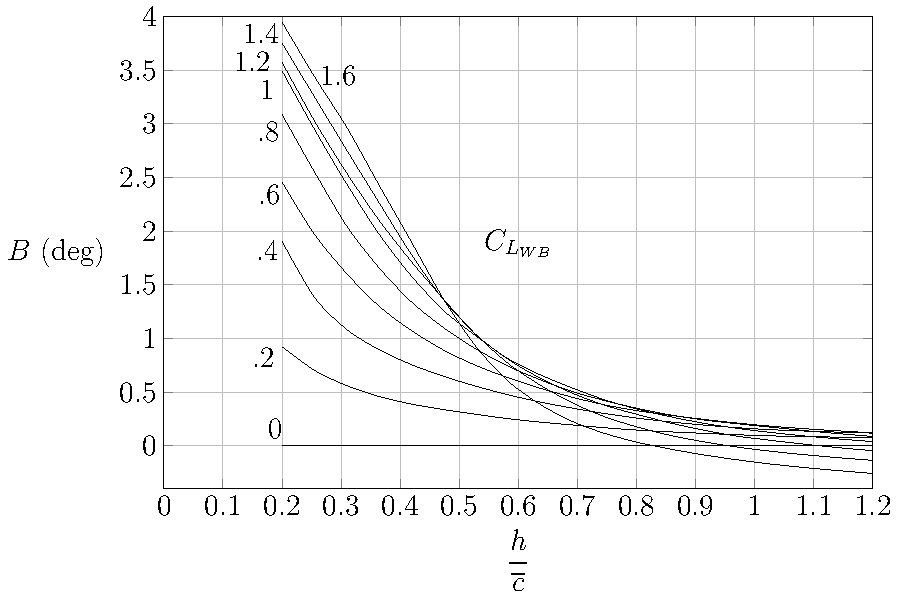
\includegraphics[height=9.5cm, keepaspectratio ]{Immagini/Capitolo2/2_14-(Delta_alpha_G)_B_vs_h_frac_overline_c_C_L_WB} 
	\caption{Parameter accounting for variation in circulation with lift and height above ground} % didascalia
	\label{fig:figura2_14} % etichetta per citarla nel testo
\end{figure}

\begin{figure}[H]
	\centering
	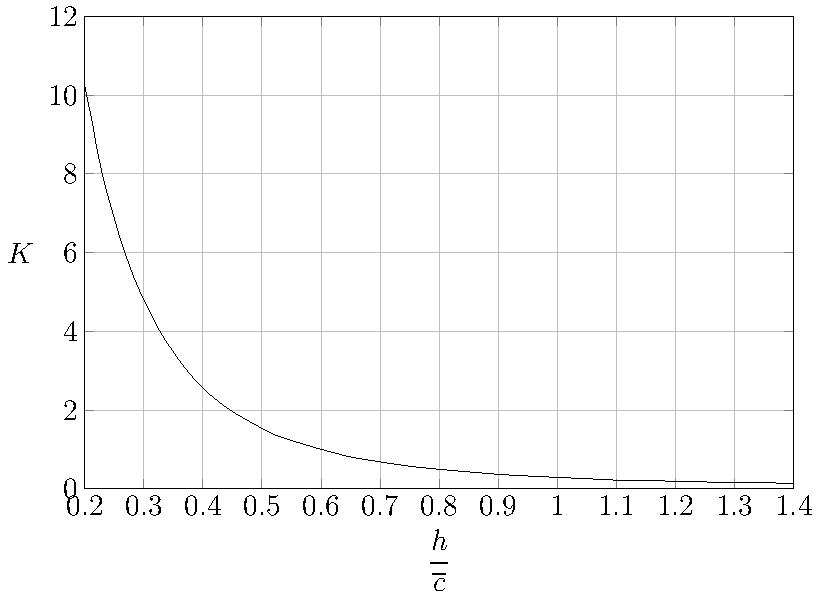
\includegraphics[height=10.5cm, keepaspectratio ]{Immagini/Capitolo2/2_15-Delta_alpha_G_K_vs_h_frac_c} 
	\caption{Parameter accounting for influence of wing thickness due to height above ground} % didascalia
	\label{fig:figura2_15} % etichetta per citarla nel testo
\end{figure}


% --------------------------------------------------------------------------------------------------------------------------------------------
% 								SEZIONE 3
% --------------------------------------------------------------------------------------------------------------------------------------------

\section{Assessment of minimum unstick speed}
The aircraft will be in the takeoff configuration at the maximum angle of attack allowed by the geometry, as shown in~\vref{fig:figura2_16}
\begin{figure}[H]
	\centering
	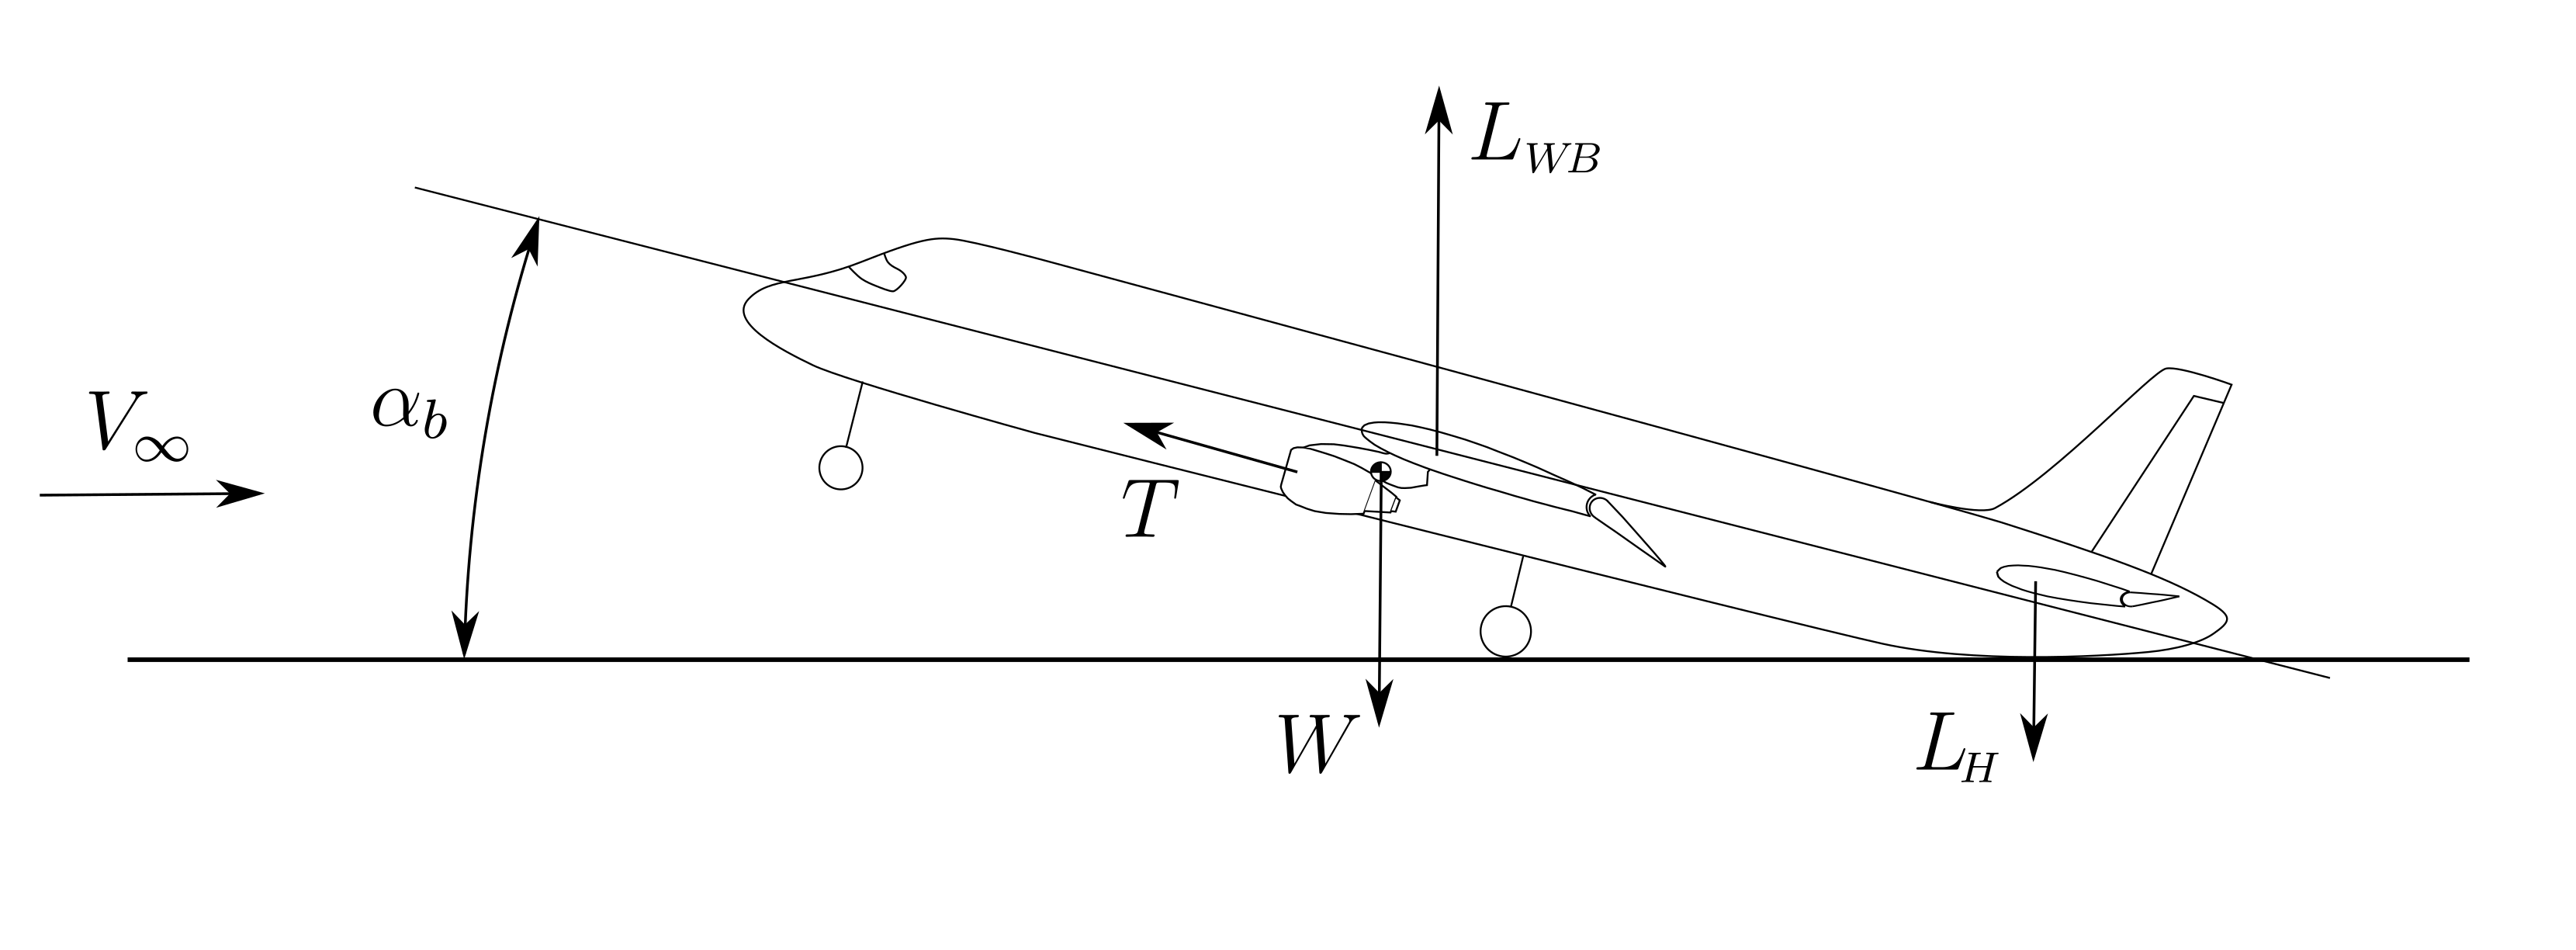
\includegraphics[height=5cm, keepaspectratio ]{Immagini/Capitolo2/2_16-aereoVmu} 
	\caption{Takeoff configuration for the assessment of VMU} % didascalia
	\label{fig:figura2_16} % etichetta per citarla nel testo
\end{figure}

Known the geometry of the fuselage can be calculated $\alpha_{W}$ and $\alpha_{H}$:

\[\alpha_{W}=\alpha_{b}+i_W\]
\[\alpha_{H}=\alpha_{b}-\varepsilon+i_H\]

The $V_{MU}$  is the speed at which the aircraft takes off in this configuration, i.e. the speed that makes the 
algebraic sum of lift (wing-body lift and horizontal tail lift) and thrust upwards component equals to the weight of the aircraft.\\
In formulas:

\begin{equation}
L_{TOT}=L_{WB}+L_H+T\sin \alpha_b=W
\label{eq:equazione2_5} % etichetta per citarla nel testo
\end{equation}
\begin{equation}
L_{TOT}=C_{L_{WB}}\frac{1}{2}\rho V_{\infty}^2S_W+C_{L_{H}}\frac{1}{2}\rho V_{\infty}^2 \eta S_H+T\sin \alpha_b=W
\label{eq:equazione2_6} % etichetta per citarla nel testo
\end{equation}
from which it is obtained:
\begin{equation}
V_{MU}=\sqrt{\frac{W-T\sin \alpha_b}{C_{L_{WB}}\frac{1}{2}\rho S_W+C{L_H}\frac{1}{2}\rho  \eta S_H}}
\label{eq:equazione2_6} % etichetta per citarla nel testo
\end{equation}
where $C_{L_{WB}}$ and $C_{L_H}$  are influenced by the ground effect. In particular there will be a new wing-body lift coefficient curve and new downwash angle as shown in section~\ref{sec:sec3}.
